\documentclass[tikz]{standalone}
\begin{document}
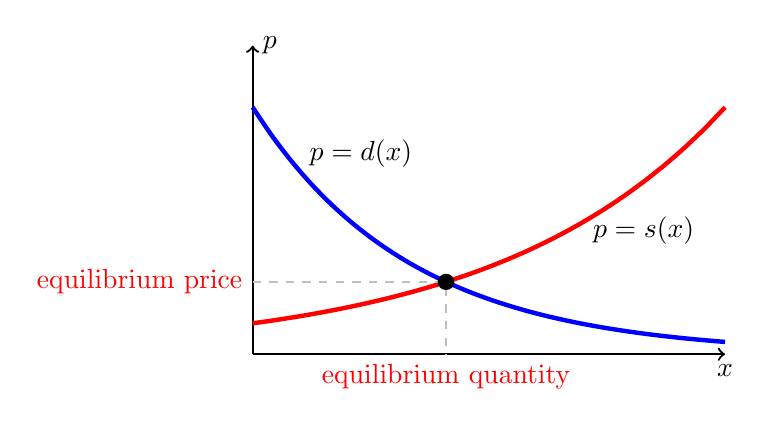
\begin{tikzpicture}[scale=2.0,yscale=0.98]
% create a white background, with a black frame
%\draw [fill=white] (-1.95,-0.35) rectangle (3.5,2.25); 

% draw axes
\draw [->,thick] (0,0) -- (3,0) node[below] {$x$}; 
\draw [->,thick] (0,0) -- (0,2) node[right] {$p$};

% plot function
\draw[ultra thick,smooth,variable=\x,blue] plot [domain=0.0:3] (\x,{1.6*exp(-\x) });
\node at (0.3,1.3) [right,black] {$p=d(x)$};
\draw[ultra thick,smooth,variable=\x,red] plot [domain=0.0:3] (\x,{0.2*pow(2.0,\x) });
\node at (2.1,0.8) [right,black] {$p=s(x)$};

% equilibrium point
\draw[lightgray,thick,dashed] (0,0.468533) -| (1.228151,0) 
node[pos=0,left,red] {equilibrium price}
node[pos=1,below,red] {equilibrium quantity};
\fill[black] (1.228151,0.468533) circle (1.5pt);

\end{tikzpicture}
\end{document}
